\documentclass[a4paper, 12pt]{report}
%\setcounter{chapter}{1}
\renewcommand\thesection{\arabic{section}}
\renewcommand{\contentsname}{Cuprins}
\renewcommand{\figurename}{Figura}
\renewcommand{\tablename}{Tabel}

\setcounter{tocdepth}{6}
\setcounter{secnumdepth}{6}

\usepackage{url}
\usepackage{hyperref}
\usepackage[backend=bibtex, style=numeric, citestyle=numeric, backref=true ,sorting=none]{biblatex}
\addbibresource{bibliography.bib}

\usepackage{indentfirst}
\usepackage[nobottomtitles*]{titlesec}

\usepackage{graphicx}
\usepackage[center]{caption}
\usepackage{caption}
\usepackage{subcaption}
\usepackage[export]{adjustbox}
\graphicspath{ {./images/} }



\usepackage[margin=3.2cm]{geometry}
%\usepackage[none]{hyphenat}

\usepackage{mathtools}

\usepackage{listings}
\usepackage{color}
\usepackage{float}

\definecolor{codegreen}{rgb}{0,0.6,0}
\definecolor{codegray}{rgb}{0.5,0.5,0.5}
\definecolor{codepurple}{rgb}{0.58,0,0.82}
\definecolor{backcolour}{rgb}{0.96,0.96,0.96}

\lstdefinestyle{mystyle}{
	backgroundcolor=\color{backcolour},   
	commentstyle=\color{codegreen},
	keywordstyle=\color{blue},
	numberstyle=\tiny\color{codegray},
	stringstyle=\color{codepurple},
	basicstyle=\fontsize{10}{10}\selectfont\ttfamily,
	breakatwhitespace=false,         
	breaklines=true,                 
	captionpos=b,                    
	keepspaces=true,                 
	numbers=left,                    
	numbersep=2pt,                  
	showspaces=false,                
	showstringspaces=false,
	showtabs=false,                  
	tabsize=2
}

\lstset{style=mystyle}

\usepackage{pythonhighlight}

\usepackage{fontspec} % -> LuaLatex
\setmainfont{UT Sans}

\usepackage{setspace}
\setstretch{1.1} % 

\begin{document}
	
	\begin{titlepage}
	
	\vspace*{-3cm}
	\hspace{-2cm}
	
\includegraphics[width=0.8\linewidth]{./images/Logo-UT-MI-SPOT-RO}

	\begin{center}
		\Huge
		
		\vspace{2cm}
		
		\textbf{Lucrare Dizertație}
		
		\vfill
				
		\Large
		\begin{tabular}{ll}
			\textbf{Autor:}&Hanganu Bogdan\\
			\textbf{Coordonator:}&Lect. Univ. Băicoianu Alexandra
		\end{tabular}
		
		\vfill
		
		\Large
		Brașov\\
		Iulie 2022
        
	\end{center}
\end{titlepage}
	\begin{titlepage}
	
	\vspace*{-3cm}
	\hspace{-2cm}
	
\includegraphics[width=0.8\linewidth]{./images/Logo-UT-MI-SPOT-RO}
	
	\begin{center}
		\Huge
		
		\vspace{2cm}
		
		\textbf{Lucrare Disertație}
		
		\vspace{1cm} 
		
		\LARGE Detectarea emoțiilor din perspective multiple
		
		\vfill
		
		\Large
		\begin{tabular}{ll}
			\textbf{Autor:}&Hanganu Bogdan\\
			\textbf{Coordonator:}&Lect. Univ. Băicoianu Alexandra
		\end{tabular}
		
		\vfill
		
		\Large
		Brașov\\
		Iulie 2022
		
	\end{center}
\end{titlepage}
	\newpage
	\tableofcontents
	\newpage
	\pagenumbering{arabic}
	\section{Abstract}	
	Această lucrare de disertație este elaborată în jurul problematicii identificării emoțiilor unei persoane. Utilizând metode de învățare automată, datele sunt înregistrate prin intermediul unor canale multiple (audio, video și text). Expresiile faciale, obținute prin intermediul canalului video, reflectă în mod intuitiv starea mentală a unei persoane, fiind una dintre cele mai bogate și importante forme de comunicare inter-umană. Tonalitatea vocii care se adresează în timpul comunicării ne poate oferi informații valoroase referitoare la starea de spirit. Mesajul care este transmis prin intermediul vocii, ne oferă informații referitoare la personalitatea individului, fiind de ajutor mai departe în procesul de analiză.
	Datele stocate sunt mai apoi prelucrate folosind tehnici de procesare specifice fiecărui canal. Pentru input-ul audio este folosită procesarea digitală de semnal, cu următoarele tehnici reprezentative: Transformata Fourier, Transformata Fourier pe termen scurt, Coeficienți Mels. Procesare de imagini pentru canalul video vine în adăugare cu: scalare de date, transformare imaginii în greyscale, iar pentru text este de menționat: tokenizare, lematizare. Fiecare bloc de date preprocesat în mod corespunzător canalului părinte, va trece mai departe prin pasul de recunoaștere cu ajutorul metodelor de învățare automată.
	În această lucrare au fost realizate o serie de experimente pentru: procesarea datelor, antrenarea modelelor de machine learning. Finalizarea acestor teste a avut ca urmare dezvoltarea aplicației "Multimodal Emotion Detection" care să vină în sprijinul procesului de intervievare.
	\clearpage
	
	\section{Introducere}
	\subsection{Interacțiunea om-mașină}
	Aplicația "Multimodal Emotion Detection" are ca audiență persoanele care doresc să facă o analiză a candidatului care a trecut printr-un proces de intervievare. Fiind scrisă în limbajul de programare Python, permite o manevrare concisă a datelor inregistrate, care pot fi mai apoi vizualizate de către utilizator prin intermediul framework-ului GUI (Graphical User Interface) QT (pronunțat "cute"). 
	
	În cadrul lucrării, se propune recunoașterea emoțiilor utilizatorului într-un mod inteligent, utilizând tehnici și metode de Machine Learning si Deep Learning. Aceste două procedee sunt subcategorii ale domeniului numit inteligență artificială, domeniu care a început să se modeleze în funcție de nevoile oamenilor.
	
	Dezvoltarea rapidă a inteligenței artificale, "Big data science" și a tehnologiei "Block chain" a provocat multiple schimbări în structura socială umană. În majoritatea proceselor unde este nevoie de interacțiune umană, se implementează automatizări care să sporească eficiența, să folosească resursele umane, software și hardware în mod cât mai eficace. La nivel industrial, sistemele automatizate inteligente sunt deja folosite in uzine, frabici, având rolul de a asigura în permanență buna funcționare a întregului ansamblu. Atât eficiența cât și performanțele acestor sisteme sunt motivate de către costul redus de mentenanță. La un nivel mai aproape de către utilizatori, putem realiza că inteligența artificială a început tot mai des să facă parte din viața de zi cu zi, ajungând în stadiul să devină indispensabil oamenilor.
	
	În zilele noastre, interacțiunea dintre oameni și I.A. este în continuă creștere, ajungand să intre treptat în viața noastră de zi cu zi. De la asistenți virtuali (care au rolul de a sprijini utilizatorul prin intermediul interpretării comenziilor vocale), până la reclame personalizate, aceste sisteme inteligente interacționează din ce în ce mai mult cu ființe umane. Deoarece este un subiect în care interesul este unul foarte crescut, relația între om și mașinăria inteligentă poate să ajungă la un nivel mai inalt, prin integrarea cu emoțiile utilizatorului. Acesta este un domeniu crucial de cercetare, oferind diverse oportunități și aplicări pentru oameni.
	
	Un aspect cheie în această sferă care să sporească parteneriatul între om și mașină este dat de înțelegerea emoțiilor umane. Emoția este un factor important atât în comunicarea verbală, cât și în comunicarea nonverbală (gesticulare, expresiile corpului). Identificarea stărilor unei persoane poate ajuta o mașină să înțeleagă intențiile utilizatorului, în scopul de a-i oferi o interacțiune mai potrivită. Printe primele studii care au fost făcute pentru integrarea sistemelor inteligente cu emoțiile umane, aceastea s-au reflectat în identificarea emoțillor prin voce, deoarece comunicarea verbala este una dintre cele mai rapide forme de socialiare, cu cel mai mare impact in istorie.
	
	Fiind una dintre cele mai consacrate aptiduni prin care o ființă inteligentă s-a putut diferenția și avansa în lanțul trofic, comunicarea verbală reprezintă un semnal complex, în care sunt transmise informații referitoare la mesaj, legate de emițător precum și de emoțiile transmise de acesta. Fiind o serie complexa, capacitatea sistemului care face identificarea emotiilor trebuie sa fie pe măsură, pentru a analiza cu acuratețe starea subiectului, oferindu-i astfel o experiență cât se poate de autentică. Nu numai atât, utilizând o astfel de recunoaștere, poate ajuta la crearea unor interfețe usor navigabile("Recunoașterea emoțiilor prin vorbire este deosebit de utilă pentru aplicațiile din domeniul interacțiunii om-mașină deoarece ajută la crearea unor interfețe usor de utilizat"\cite{emotion_recognition_survery}).
	
	Deoarece semnalul audio conține și alte informații precum emoția transmisă de către emițător, algortimul de recunoaștere a emoțiilor umane prin extragerea trăsăturilor acustice capturate în vorbire, devine "baza pentru realizarea unei interacțiuni om-calculator mai armonioasă și mai eficientă, având o mare importanță în cercetare, precum și aplicativă"\cite{audio_emotion_recognition0}.
	
	În cadrul aplicației, vocea utilizatorului (semnalul audio) este folosită în doua contexte. Primul este dat de către identificarea emoțiilor candidatului pe baza a diferite trăsături acustice depistate din voce iar al doilea de către identificarea cuvintelor rostite, pentru a putea fi transformate în text. Deoarece în aplicatie identificarea textului (speech-to-text) este utilizat prin intermediul unor apeluri de tip API Rest la functionalitățile oferite de către Google, accentul se va pune pe prima utilizare în lucrare.
	
	% Diacritice
	% Introducere emotion recognition text
	Seviciului oferit de catre Google pentru recunoasterea textului este folosit cu scopul de a permite o captare a dialogului avut
	
	% Introducere emotion recognition video
	
	
	% Descriere despre produs finit
	% Descriere alte tipuri de emotion recognition (Human body gesture)
	% Alte tipuri de aplicatii similare + 2 exemple
	% Utilitate
	% Structurare lucrarii
	\subsection{}
	\clearpage
	
   \printbibliography
   \clearpage
   %\lstlistoflistings
	\begin{figure}[H]
		\begin{center}
			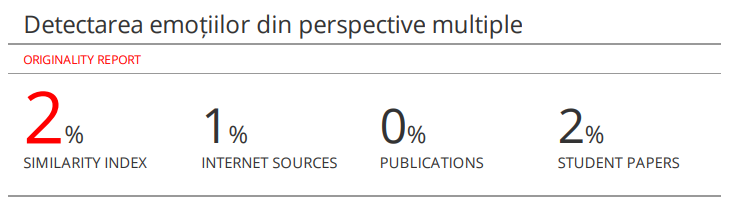
\includegraphics[scale=0.4]{images/plagiat.PNG}
		\end{center}
		\caption{Licență similaritate}
		\label{fig:sim}
	\end{figure} 	
\end{document}